%
% performance_analyis.tex
%
% Copyright (C) 2019 by Gabriel Mariano Marcelino <gabriel.mm8@gmail.com>.
%
% Relatório final do Trabalho Final da Disciplina EEL510265.
%
% This work is licensed under the Creative Commons Attribution-ShareAlike 4.0
% International License. To view a copy of this license,
% visit http://creativecommons.org/licenses/by-sa/4.0/.
%

%
% \brief Performance analysis section.
%
% \author Gabriel Mariano Marcelino <gabriel.mm8@gmail.com>
%
% \version 0.1.0
%
% \date 27/11/2019
%

\section{Análise de Desempenho} \label{sec:performance-analysis}

Utilizando a ferramenta ``\textit{top}'' do Linux, é possível ter uma estimativa do consumo de recursos do \textit{software} desenvolvido. Os resultados obtidos podem ser vistos na \autoref{fig:top-results}.

\begin{figure}[!ht]
    \begin{center}
        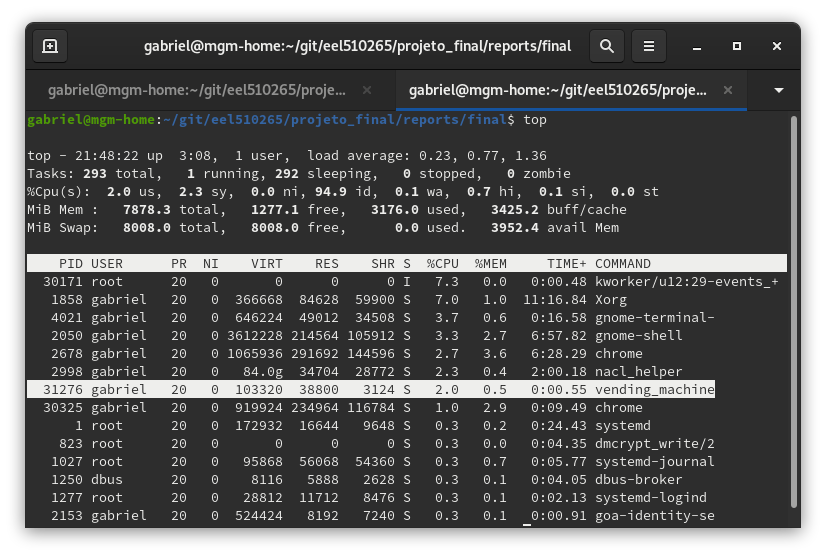
\includegraphics[width=\textwidth]{figures/top-output.png}
        \caption{Consumo de recursos utilizando a ferramenta ``\textit{top}'' (linha destacada no centro da imagem).}
        \label{fig:top-results}
    \end{center}
\end{figure}

Nessa captura de tela, pode-se ver o uso do processador em 2 \% e aproximadamente 103 MB de paǵinas de memória alocadas.

Para se obter uma medida mais próxima ao consumo real de memória, utilizou-se a ferramenta ``\textit{Valgrind}'' \footnote{\href{http://valgrind.org/}{http://valgrind.org/}}. Esta ferramenta é um \textit{framework} de instrumentação para análise dinâmica de aplicações de \textit{software}. Para mensurar o consumo de memória, utilizou-se um \textit{profiler} de memória \textit{heap}. Um gráfico com os resultados obtidos pode ser visto na \autoref{fig:mem-usage}.

\begin{figure}[!ht]
    \begin{center}
        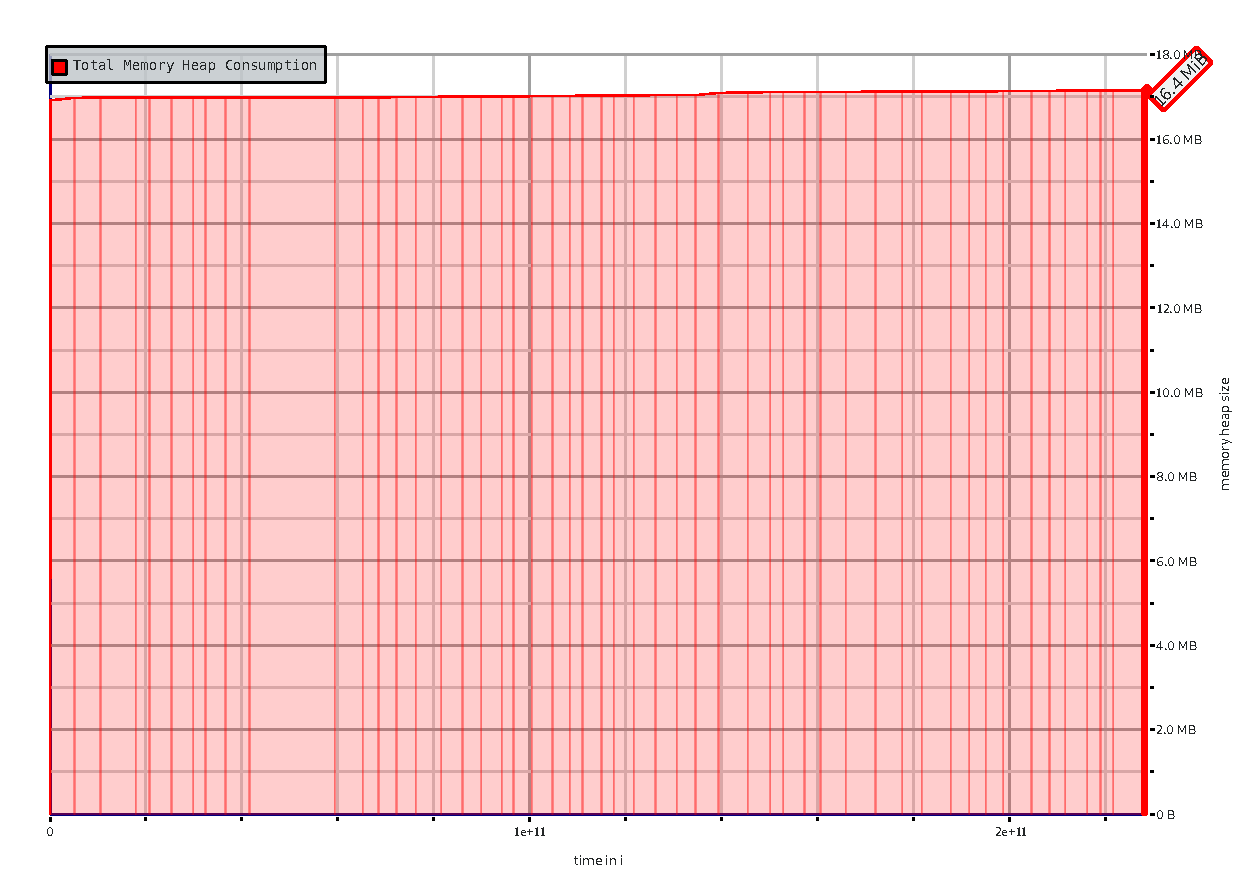
\includegraphics[width=\textwidth]{figures/mem-usage.pdf}
        \caption{Consumo de memória medido.}
        \label{fig:mem-usage}
    \end{center}
\end{figure}

Como é possível observar na \autoref{fig:mem-usage}, o consumo de memória do \textit{software} estabilizou em aproximadamente 16,4 MiB. Este gráfico foi obtido com o auxílio da ferramenta ``\textit{massif-visualizer}''\footnote{\href{https://github.com/KDE/massif-visualizer}{https://github.com/KDE/massif-visualizer}}, que permite a visualização na forma de gráficos dos resultados gerados pela ferramenta ``massif'' do ``Valgrind''.
